\section{Problem (6)}
	In the \cref{fig:hw9_problem6}, block $A$ (mass $1.5 \ sl$) slides into block $B$ (mass $2.5 \ sl$), along a frictionless surface. The directions of velocities before and after the collision are indicated; the corresponding speeds are $v_{Ai} = \ 4.0 \ ft/s$, $v_{Bi} = \ 2.4 \ ft/s$, and $v_{Bf} = \ 3.2 \ ft/s$. What is velocity $v_{Af}$ (including sign, where positive denotes motion to the right)?

	\begin{figure}[H]
		\begin{center}
			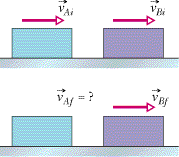
\includegraphics[scale=1]{hw9_problem6}
			\caption{Illustration of Problem 6}
			\label{fig:hw9_problem6}
		\end{center}
	\end{figure}

	\textbf{R:}

	\begin{align}
		\Delta p = \ &0& \notag \\
		p_{i} = \ &p_{f}& \notag \\
		m_{A}\vec{v}_{Ai} + m_{B}\vec{v}_{Bi} = \ &m_{A}\vec{v}_{Af} + m_{B}\vec{v}_{Bf}& \notag \\
		\vec{v}_{Af} = \ &\frac{m_{A}\vec{v}_{Ai} + m_{B}\vec{v}_{Bi} - m_{B}\vec{v}_{Bf}}{m_{A}}& \notag \\
		= \ &\vec{v}_{Ai} + \frac{m_{B}(\vec{v}_{Bi} - \vec{v}_{Bf})}{m_{A}}& \notag \\
		= \ &(4.0 \ ft/s) + \frac{(2.5 \ sl)[(2.4 \ ft/s) - (3.2 \ ft/s)]}{1.5 \ sl}& \notag \\
		= \ &(4.0 \ ft/s) + (1.\bar{6})(-0.8 \ ft/s)& \notag \\
		= \ &(4.0 \ ft/s) - (1.\bar{3} \ ft/s)& \notag \\
		= \ &+ 2.\bar{6} \ ft/s&
	\end{align}
